

\twocolumn[\centerline {\textsc{\LARGE
ОТВЕТЫ,\hspace{0.5em}УКАЗАНИЯ,\hspace{0.5em}РЕШЕНИЯ}}]
\rule{\textwidth}{1 pt}
\medskip
{\textsc{\large<<КВАНТ>> ДЛЯ МЛАДШИХ ШКОЛЬНИКОВ}

\par \medskip  ЗАДАЧИ}

{\it (см. <<Квант>> №5)}

\begin{enumerate}[itemsep = -3pt, itemindent = -7pt, labelsep = 5pt, font = \bfseries, topsep = 3pt, wide]
    \item Заднее колесо трактора за секунду совершит ровно 1 оборот.
    \item См. таблицу:
\begin{table}[h]
\centering
    \begin{tabular}{|m{4ex}|m{4ex}|m{4ex}|m{4ex}|m{4ex}| m{4ex}|}
    \hline
         \cellcolor{lightgray} & 7<<А>> & 7<<Б>> & 7<<В>> & 7<<Г>> & $\sum$ \\
         \hline
        7<<А>> & \cellcolor{lightgray} & 3:0 & 2:1 & 2:0 & 7:1 \\ 
        \hline
        7<<Б>> & 0:3 & \cellcolor{lightgray} & 0:0 & 2:0 & 2:3 \\ 
        \hline
        7<<В>> & 1:2 & 0:0 & \cellcolor{lightgray} & 2:1 & 3:3 \\ 
        \hline
        7<<Г>> & 0:2 & 0:2 & 1:2 & \cellcolor{lightgray} & 1:6 \\ 
        \hline
    \end{tabular}
\end{table}
    \item Обозначим угол AOB через $\alpha$, тогда \angle AOB $= \frac{\alpha}{2}$, а \angle DOC $= \frac{\pi}{2} = \frac{\alpha}{2}$. Угол COB равен  $\alpha = \frac{\pi}{2}$, а \angle COE $= \frac{\alpha}{2} = -\frac{\pi}{4}$.  Следовательно \angle DOE = \angle DOC + \angle COE = $\left(\frac{\pi}{2} - \frac{\alpha}{2}\right) + \left(\frac{\alpha}{2} - \frac{\pi}{4}\right) = \frac{\pi}{4}$.
    \medskip
    \item Разобьем гирьки на 50 пар соседних гирек. Затем эти 50 пар разобьем на две кучки по 25 пар. Теперь из первой кучки положим на левую чашку весов более тяжелую гирьку из каждой пары, а на правую - более легкую. Со второй кучкой поступим наоборот - на левую чашку положим более легкие гирьки из пар, а на правую - более тяжелые. Очевидно, что в результате весы окажутся в равновесии.
    \item Судья не всегда может сделать расписание на оставшиеся 2 дня. Например, если в первые три дня команды играли 
       \vspace{-0.75cm}
   \begin{figure}[h]
   \centering
       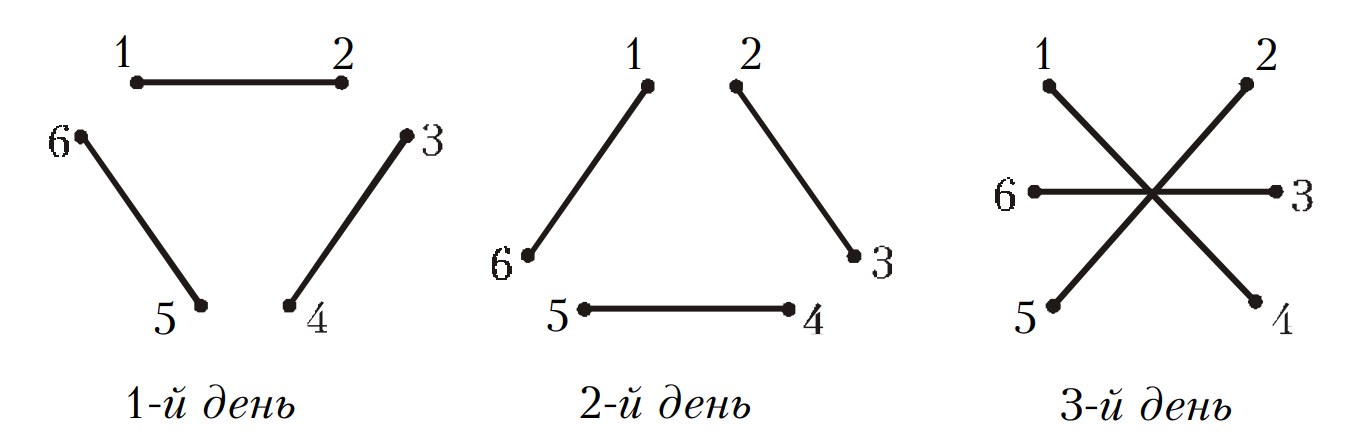
\includegraphics[scale = 0.18]{Матчи.png}
       \captionsetup{justification=raggedright,
singlelinecheck=false}
       \caption{}
   \end{figure}
   \vspace{-0.5cm}
    так, как показано на рисунке 1 (отрезками соеденены номера команд, играющих в этот день), невозможно было бы устроить расписание даже только на четаертый день. Действительно, команда с нечетным номером может играть лишь с командами, имеющими нечетнве номера, но таких команд три, следовательно, одной из них не с кем будет играть в четвертый
    \medskip
    
    {\it (см. <<Квант>> №6)}
\end{enumerate}

\begin{enumerate}[itemsep = -3pt, itemindent = -7pt, labelsep = 5pt, font = \bfseries, topsep = 3pt, wide]
\item Смогут. Поскольку Буратиноне хватает 18 сольдо, а Мальвине не хватает 7 сольдо, у Мальвины есть по крайней мере $18 - 7 = 11$  сольдо. Если она добавит их к деньгам Пьеро, то денег на букварь, конечно же, хватит.
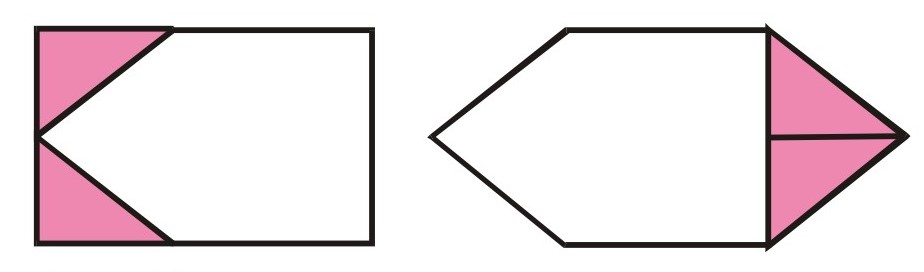
\includegraphics[width=0.3\textwidth]{Ромбики1jpg.jpg}%
\parbox[b]{0.185\textwidth}{\item \smallskip См. рис. 2, 3.\item Число 220 нельзя представить в виде суммы двух натуральных чисел, все цифры}
\vspace{-12pt}
\begin{flushleft}
 \quad Рис. 2
\end{flushleft}
\vspace{-10pt}
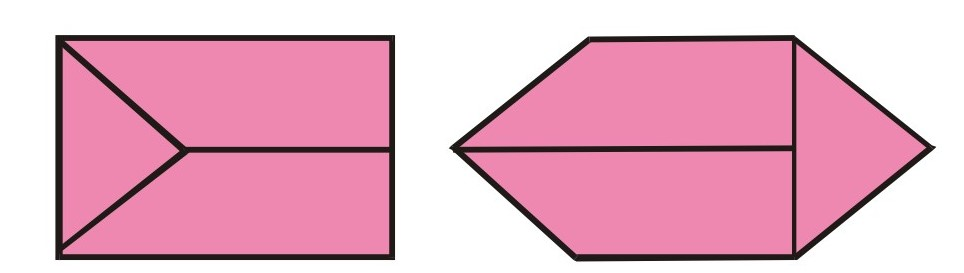
\includegraphics[width=0.3\textwidth]{Ромбики2jpg.jpg}%
\parbox[b]{0.185\textwidth}{которых нечетны.\vspace{1mm}\item 1665. Сумма последних трехцифр исходных трехзначных чисел оканчивается на 5.Числа 5 и 25 не представимы в виде суммы трех ненулевых}
\vspace{-10pt}
\\ \\
различных цифр. Значит сумма последних чисел равна 15. Тогда сумма средних чисел тоже равна 15, и суммма первых чисел тоже 15. Теперь ясно, что после перестановки \\ \parbox[b]{0.185\textwidth}{ мы получим три числа, сумма которых 1665. \\ Напоследок предъявим тройку чисел(одну из возможных), которая удовлетворяем условию задачи: 159, 672, 834. \item  На рисунке 4 король сделал 49 диагональных ходов. Доказать, что число 49 максимально возможное, очень просто.}
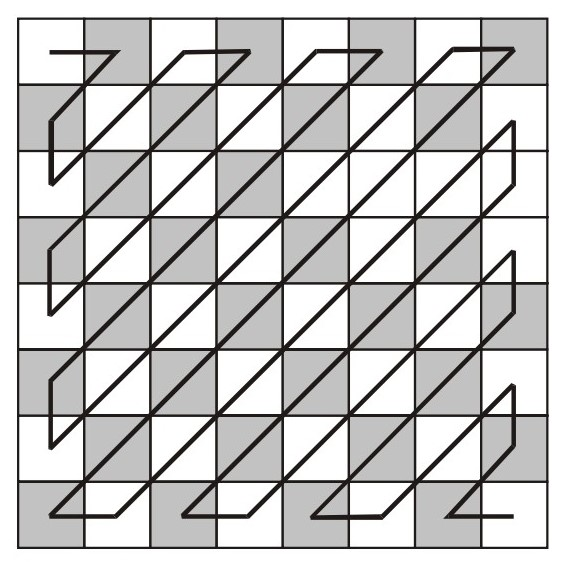
\includegraphics[width=0.3\textwidth]{Доска.jpg} 
\vspace{-0.8cm}
\begin{center}
    Рис. 4
\end{center} \\
\vspace{-0.45cm}
Каждый диагональный ходпроходит через один узел шахматной доски. (Узлом мы здесь называем общую точку 4 клеток шахматной доски.) Всего узлов 49.Два раза пройти через один и тот же узел без самопересечения пути невозможно.
\end{enumerate}
\medskip

{\textsc{\Large МЕТАМОРФОЗЫ ПОСЛЕДОВАТЕЛЬНОСТЕЙ}}

\begin{enumerate}[itemsep = -3pt, itemindent = -7pt, labelsep = 5pt, font = \bfseries, topsep = 3pt, wide]
\item П$_9$, П$_{10}$, П$_{11}$. Если считать, что в момент отплытия лодки отправляется автобус №0, то турист должен сесть в автобус  №66. (Решение аналогичной задачи см. на с. 87-88 в журнале <<Квант>> №1/2 за 1993 г.)
\item $P_4(x) = x^4 + 2x^3 + x^2 - \frac{1}{30}$,\\
{\small $S_4(n) = \frac{1}{5}n^5 + \frac{1}{2}n^4 + \frac{1}{3}n^3 - \frac{1}{30}n = \frac{n(n+1)(2n + 1)(3n^2+3n -1)}{30}$.}
\item $S_k(0) = \int_{0}^{0}P_k(x)dx = 0$.
\item {\it Указание.} Коэффицент при старшей степени многочлена P$_k$(x) равен 1.\\
\item $-\frac{1}{2} + \frac{(-1)^n}{2cos\frac{1}{2}} cos\left(n  + \frac{1}{2}\right)$.
\end{enumerate}\\
{\it Указание.}

 \qquad $\sum_{k = 1}^{n} (-1)^k cosk = \frac{1}{2}\sum_{k=1}^{n} \left((cos(\pi + 1)k +cos(\pi - 1)k \right)$
 
\medskip
{\textsc{\Large АНАЛОГИИ В ЗАДАЧАХ ПО ФИЗИКЕ}}

\begin{enumerate*} [itemsep = -3pt, itemindent = -7pt, labelsep = 5pt, font = \bfseries, topsep = 3pt]
    \item $T = \frac{kq\lambda}{R}$.\qquad
    \item $T = \sigma R$.
    \item[3, 4, 5.] $\Delta W = - W_0/2$.
\end{enumerate*}

\medskip
{\textsc{\Large МОСКОВСКИЙ ФИЗИКО-ТЕХНИЧЕСКИЙ ИНСТИТУТ}}

{\rmfamily{\large МАТЕМАТИКА}}

Вариант 1

\begin{enumerate}[itemsep = -3pt, itemindent = -7pt, labelsep = 5pt, font = \bfseries, topsep = 3pt, wide]
    \item $x = \ps \frac{3\pi}{4} + 2\pi k, k \in {\bf Z}$. {\it Указание.} В каждом из случаев $cosx < 0$ и $cosx > 0$ выполните подстановку $\frac{cos3x}{cosx}$.
    \item $x < \frac{34 - 30\sqrt{2}}{23}, x \geq 3$.
    \item $\frac{5\sqrt{34}}{12}$. Решение. Точка D является центром описанной около треугольника  ABC окружности, AB = 5, AC = 4. Пусть О$_1$ -- центр окружности, вписанной в равнобедренный треугольник BCD. O$_2$ -- цент окружности, описанной около равнобедренного треугольника ACD, M --  середина отрезка CB (рис. 5) ...
\end{enumerate}
